\documentclass[xelatex,a5paper,ja=standard, openany]{bxjsbook}

% 各種パッケージ
\usepackage{graphicx} % figure環境
\usepackage{titlesec}
\usepackage{hyperref}

\usepackage{noto}
\usepackage[T1]{fontenc} % 欧文フォント変えるときのおまじない


\usepackage{listings}
\renewcommand{\lstlistingname}{ソースコード}

\lstset{
    basicstyle={\ttfamily\gtfamily\scriptsize},
    identifierstyle={},
    commentstyle={},
    keywordstyle={\bfseries},
    ndkeywordstyle={},
    stringstyle={\ttfamily},
    frame={tb},
    breaklines=true,
    columns=[l]{fullflexible},
    numbers=left,
    numberstyle={\ttfamily\tiny},
    stepnumber=1,
    tabsize=4,
    keywordstyle={},     %キーワード(int, ifなど)の書体指定
    commentstyle={},  %注釈の書体
    stringstyle={},        %文字列
    showstringspaces=false,  %文字列中の半角スペースを表示させない
    keepspaces=true,
}


\pagestyle{headings}

% chapter
\titleformat{\chapter}[block]
{\bfseries\gtfamily\sffamily\Huge}
{\Large 第\thechapter 章\\\Huge}{0pt}
{}
[\titlerule]

\titlespacing*{\chapter}{0pt}{0em}{1.5em}[0pt] % 余白指定

% section
\titleformat{\section}[block]
{\bfseries\gtfamily\sffamily\Large}
{\thesection}{10pt}
{}
[\titlerule]

% subsection
\titleformat{\subsection}[block]
{\bfseries\gtfamily\sffamily\large}
{\thesubsection}{10pt}
{}
[\titlerule]


\title{}
\author{} 
\date{}

\begin{document}
\tableofcontents

\chapter{CPUの概要}

CPUの基板をご購入いただきありがとうございます。と説明書っぽいことを言ってみる。まあ書くこともないし、紙が無駄なのでこれぐらいにする。

\section{基板}

\begin{figure}[h]
    \centering
    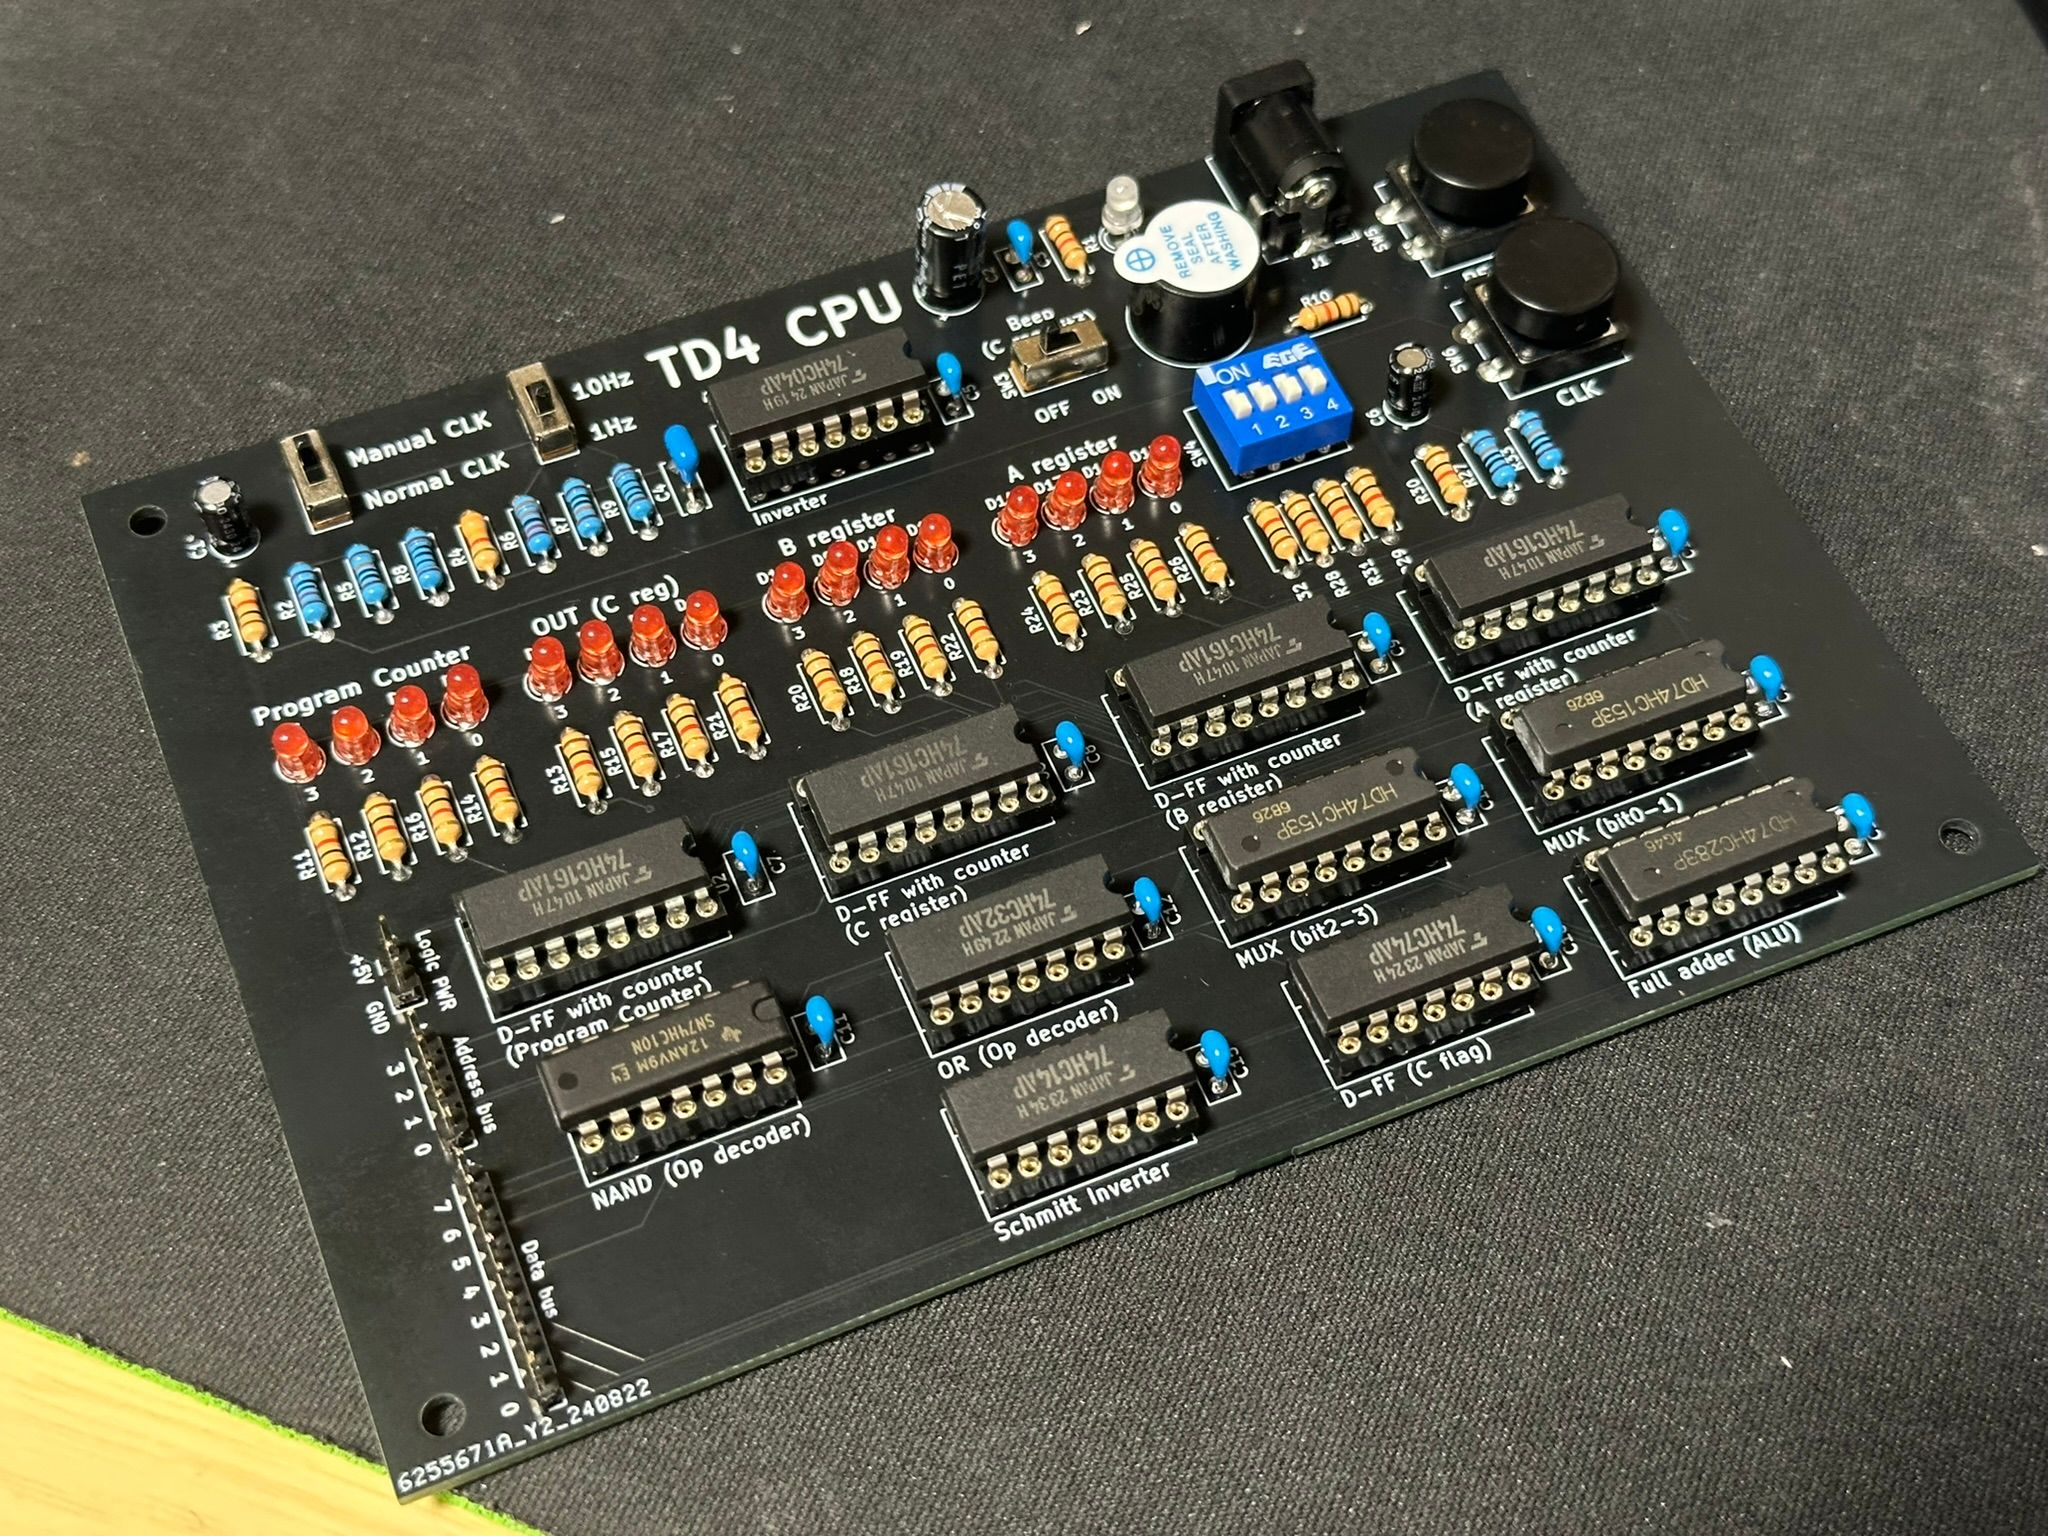
\includegraphics[width=0.6\linewidth]{figure/kiban.jpeg}
    \caption{完成した基板}
    \label{fig:kanseikiban}
\end{figure}

このCPUは、書籍「CPUの創りかた\footnote{\texttt{\url{https://book.mynavi.jp/ec/products/detail/id=22065} (ISBN4-8399-0986-5)}}」で製作するTD4 CPUの回路を、筆者が基板に起こしたものになる。\par
書籍ではユニバーサル基板上に配線していたが、そんなことしたくなかったので基板を作ることにした。基板設計など一切したことなかったので、専門家が見たら怒る点もあると思うが、気にしないでほしい。
部品を実装すれば動くと思うが、書籍も参照しながら作ることをおすすめする。\par

基板の設計はKiCad 8.0を利用した。無料のCADだが非常に使いやすかった。また、基板はJLCPCBに発注した。
\section{CPU}
CPUの概要を以下に示す。

\begin{itemize}
    \item 命令データ長 8bit
    \item アドレスバス長 4bit
    \item 2つの4bitレジスタ(A,B)
    \item 4bit 入出力 (IN, OUT)
    \item 4bit プログラムカウンタ
    \item ALUは全加算器のみ
\end{itemize}

命令フォーマットは、図\ref{fig:op_format}のように、上位4bitが命令コード、下位4bitがイミディエイトデータの計8bit構成となっている。
\begin{figure}[h]
    \centering
    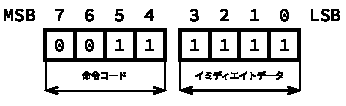
\includegraphics[width=0.8\linewidth]{figure/td4cpu_op.pdf}
    \caption{命令フォーマット}
    \label{fig:op_format}
\end{figure}

\newpage
命令コードの一覧と意味、ニーモニックを表\ref{table:opcode_list}に示す。

\begin{table}[h]
    \centering
    \begin{tabular}{lll}
        ニーモニック                   & 命令コード                  & 意味                                       \\
        \hline
        \texttt{MOV A, {[}Im{]}} & \texttt{0011 {[}Im{]}} & A\textleftarrow Im                       \\
        \texttt{MOV B, {[}Im{]}} & \texttt{0111 {[}Im{]}} & B\textleftarrow Im                       \\
        \texttt{MOV A, B}        & \texttt{0001 0000}     & A\textleftarrow B                        \\
        \texttt{MOV B, A}        & \texttt{0100 0000}     & B\textleftarrow A                        \\
        \texttt{ADD A, {[}Im{]}} & \texttt{0000 {[}Im{]}} & A\textleftarrow A + Im                   \\
        \texttt{ADD B, {[}Im{]}} & \texttt{0101 {[}Im{]}} & B\textleftarrow B + Im                   \\
        \texttt{IN A}            & \texttt{0010 0000}     & A\textleftarrow IN                       \\
        \texttt{IN B}            & \texttt{0110 0000}     & B\textleftarrow IN                       \\
        \texttt{OUT {[}Im{]}}    & \texttt{1011 {[}Im{]}} & OUT\textleftarrow Im                     \\
        \texttt{OUT B}           & \texttt{1001 {[}Im{]}} & OUT\textleftarrow Im                     \\
        \texttt{JMP {[}Im{]}}    & \texttt{1111 {[}Im{]}} & PC\textleftarrow Im                      \\
        \texttt{JNC {[}Im{]} }   & \texttt{1110 {[}Im{]}} & if (C is not 1) then PC\textleftarrow Im
    \end{tabular}
    \caption{命令コードの一覧}
    \label{table:opcode_list}
\end{table}

\chapter{製作}
CPUの概要や回路を説明するのは書籍に任せるとして、この基板の製作について述べる。

\section{部品表}
基板以外に別途、別紙1に示した部品が必要となる。部品は必要個数のみ表記しているので、予備も含めて買うのをお勧めする。\par

部品については秋月電子通商\footnote{\url{https://akizukidenshi.com/catalog/default.aspx}}と樫木総業株式会社\footnote{\url{https://www.kashinoki.shop/}}ですべて購入できる。秋月電子通商で買える部品については秋葉原店の店頭ですべて購入できた(2024年8月現在)。\texttt{74HC14}だけバックヤードにあるためレジで店員に言わなければならないので注意。\par

秋葉原には秋月以外にもマルツや千石通商など、電子部品の店が多くある。この機会に秋葉原に出向いて色々なお店を見ながら選ぶと楽しいと思う。

\section{部品の実装}
はんだごて片手にひたすらはんだ付けする。表面実装部品は無いのではんだ付けの難易度は低いと思う。ただ量が多い。\par
暇だったのでアニメを見ながらはんだ付けをしていた。\par
このCPUの製作ではんだ付けを初めて行うという人は、はんだ付けの動画などを見て学ぶことをお勧めする。くれぐれも火傷には気を付けてほしい。


\subsection{注意点}
部品実装の注意点としては、電解コンデンサ(MLCCと書いていないもの)は極性\footnote{簡単に言えば部品のプラスマイナスの向きのこと。逆につなぐと爆発などの危険がある}がある。

\begin{figure}[ht]
    \centering
    \begin{minipage}[t]{0.45\linewidth}
        \centering
        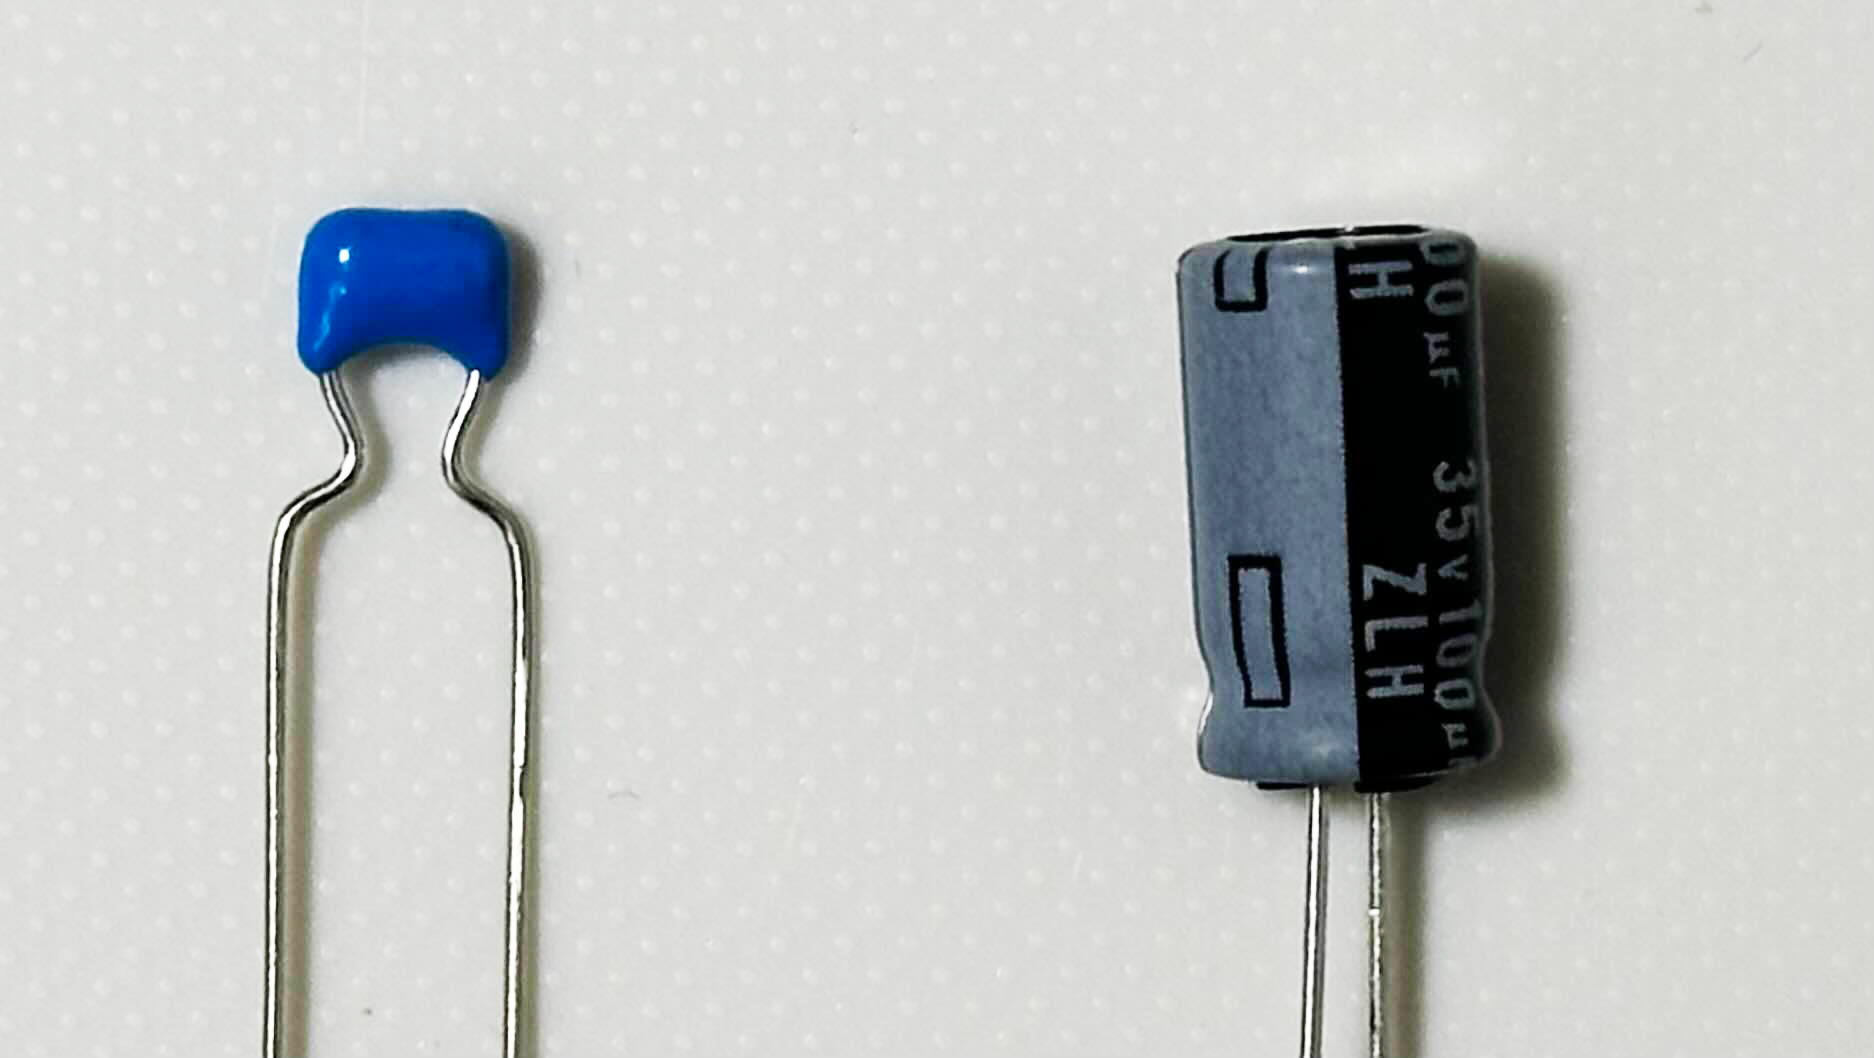
\includegraphics[keepaspectratio, width=\linewidth]{figure/capacitor.png}
        \caption{積層セラミックコンデンサ(左)と電解コンデンサ(右)}
        \label{fig:capacitor}
    \end{minipage}
    \begin{minipage}[t]{0.45\linewidth}
        \centering
        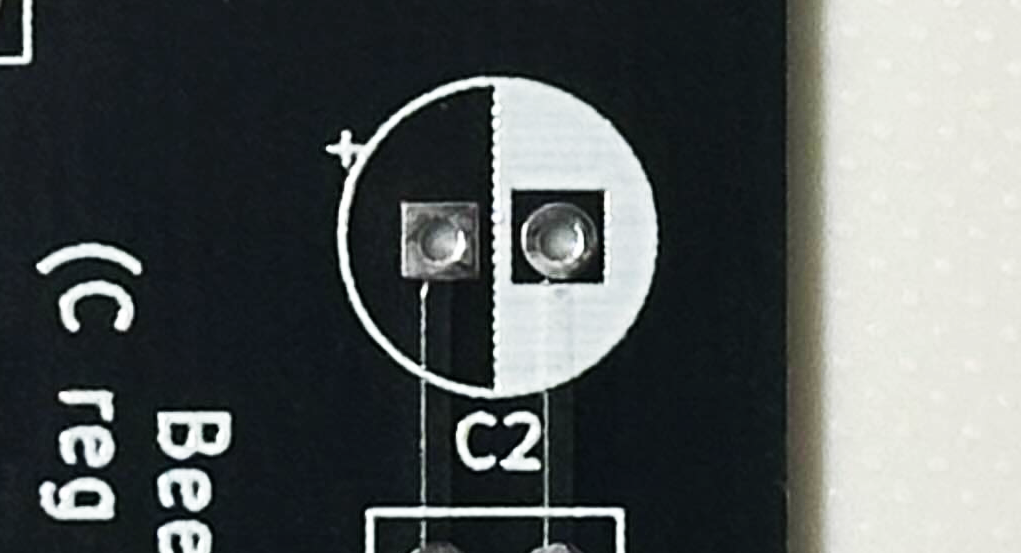
\includegraphics[keepaspectratio, width=\linewidth]{figure/kiban_capacitor.png}
        \caption{基板上の電解コンデンサの表記}
        \label{fig:capacitor_kiban}
    \end{minipage}
\end{figure}

電解コンデンサを見ると半分が白くなっていて、でかでかと-(マイナス)が書かれていると思う。これと基板上の白い部分の向きを合わせれば問題ない。また、積層セラミックコンデンサについては極性はない。\par

\hrulefill

\begin{figure}[h]
    \centering
    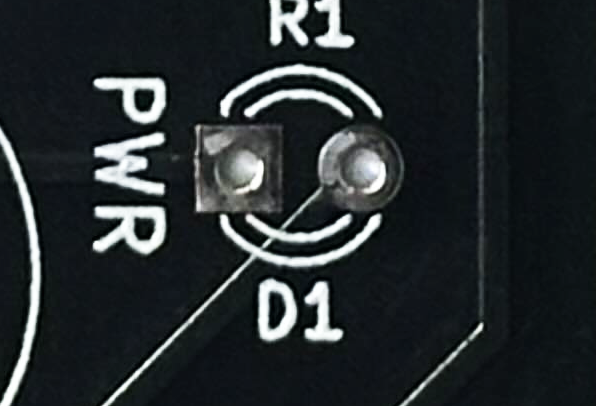
\includegraphics[width=0.3\linewidth]{figure/led_kiban.png}
    \caption{基板上のLEDの表記}
    \label{fig:led_kiban}
\end{figure}

電源やレジスタの値の表示用にLED(発光ダイオード)を利用している。これも極性があるので注意してほしい。部品を刺す穴の周りの金属が四角いほう(図\ref{fig:led_kiban}では左側)がマイナス(LEDの足が短い方)になる。最悪こちらは逆につないでも光らないだけで回路に影響は無いはず。

ICは印刷されている切り欠きとICの切り欠きを合わせて差し込むようにする。逆だと正しく動かなかったり、ICを壊す可能性もある。というか絶対に壊す。ICソケットを使用する場合はICソケットにも切り欠きがあるので合わせるのが良い。

\begin{figure}[ht]
    \centering
    \begin{minipage}[t]{0.4\linewidth}
        \centering
        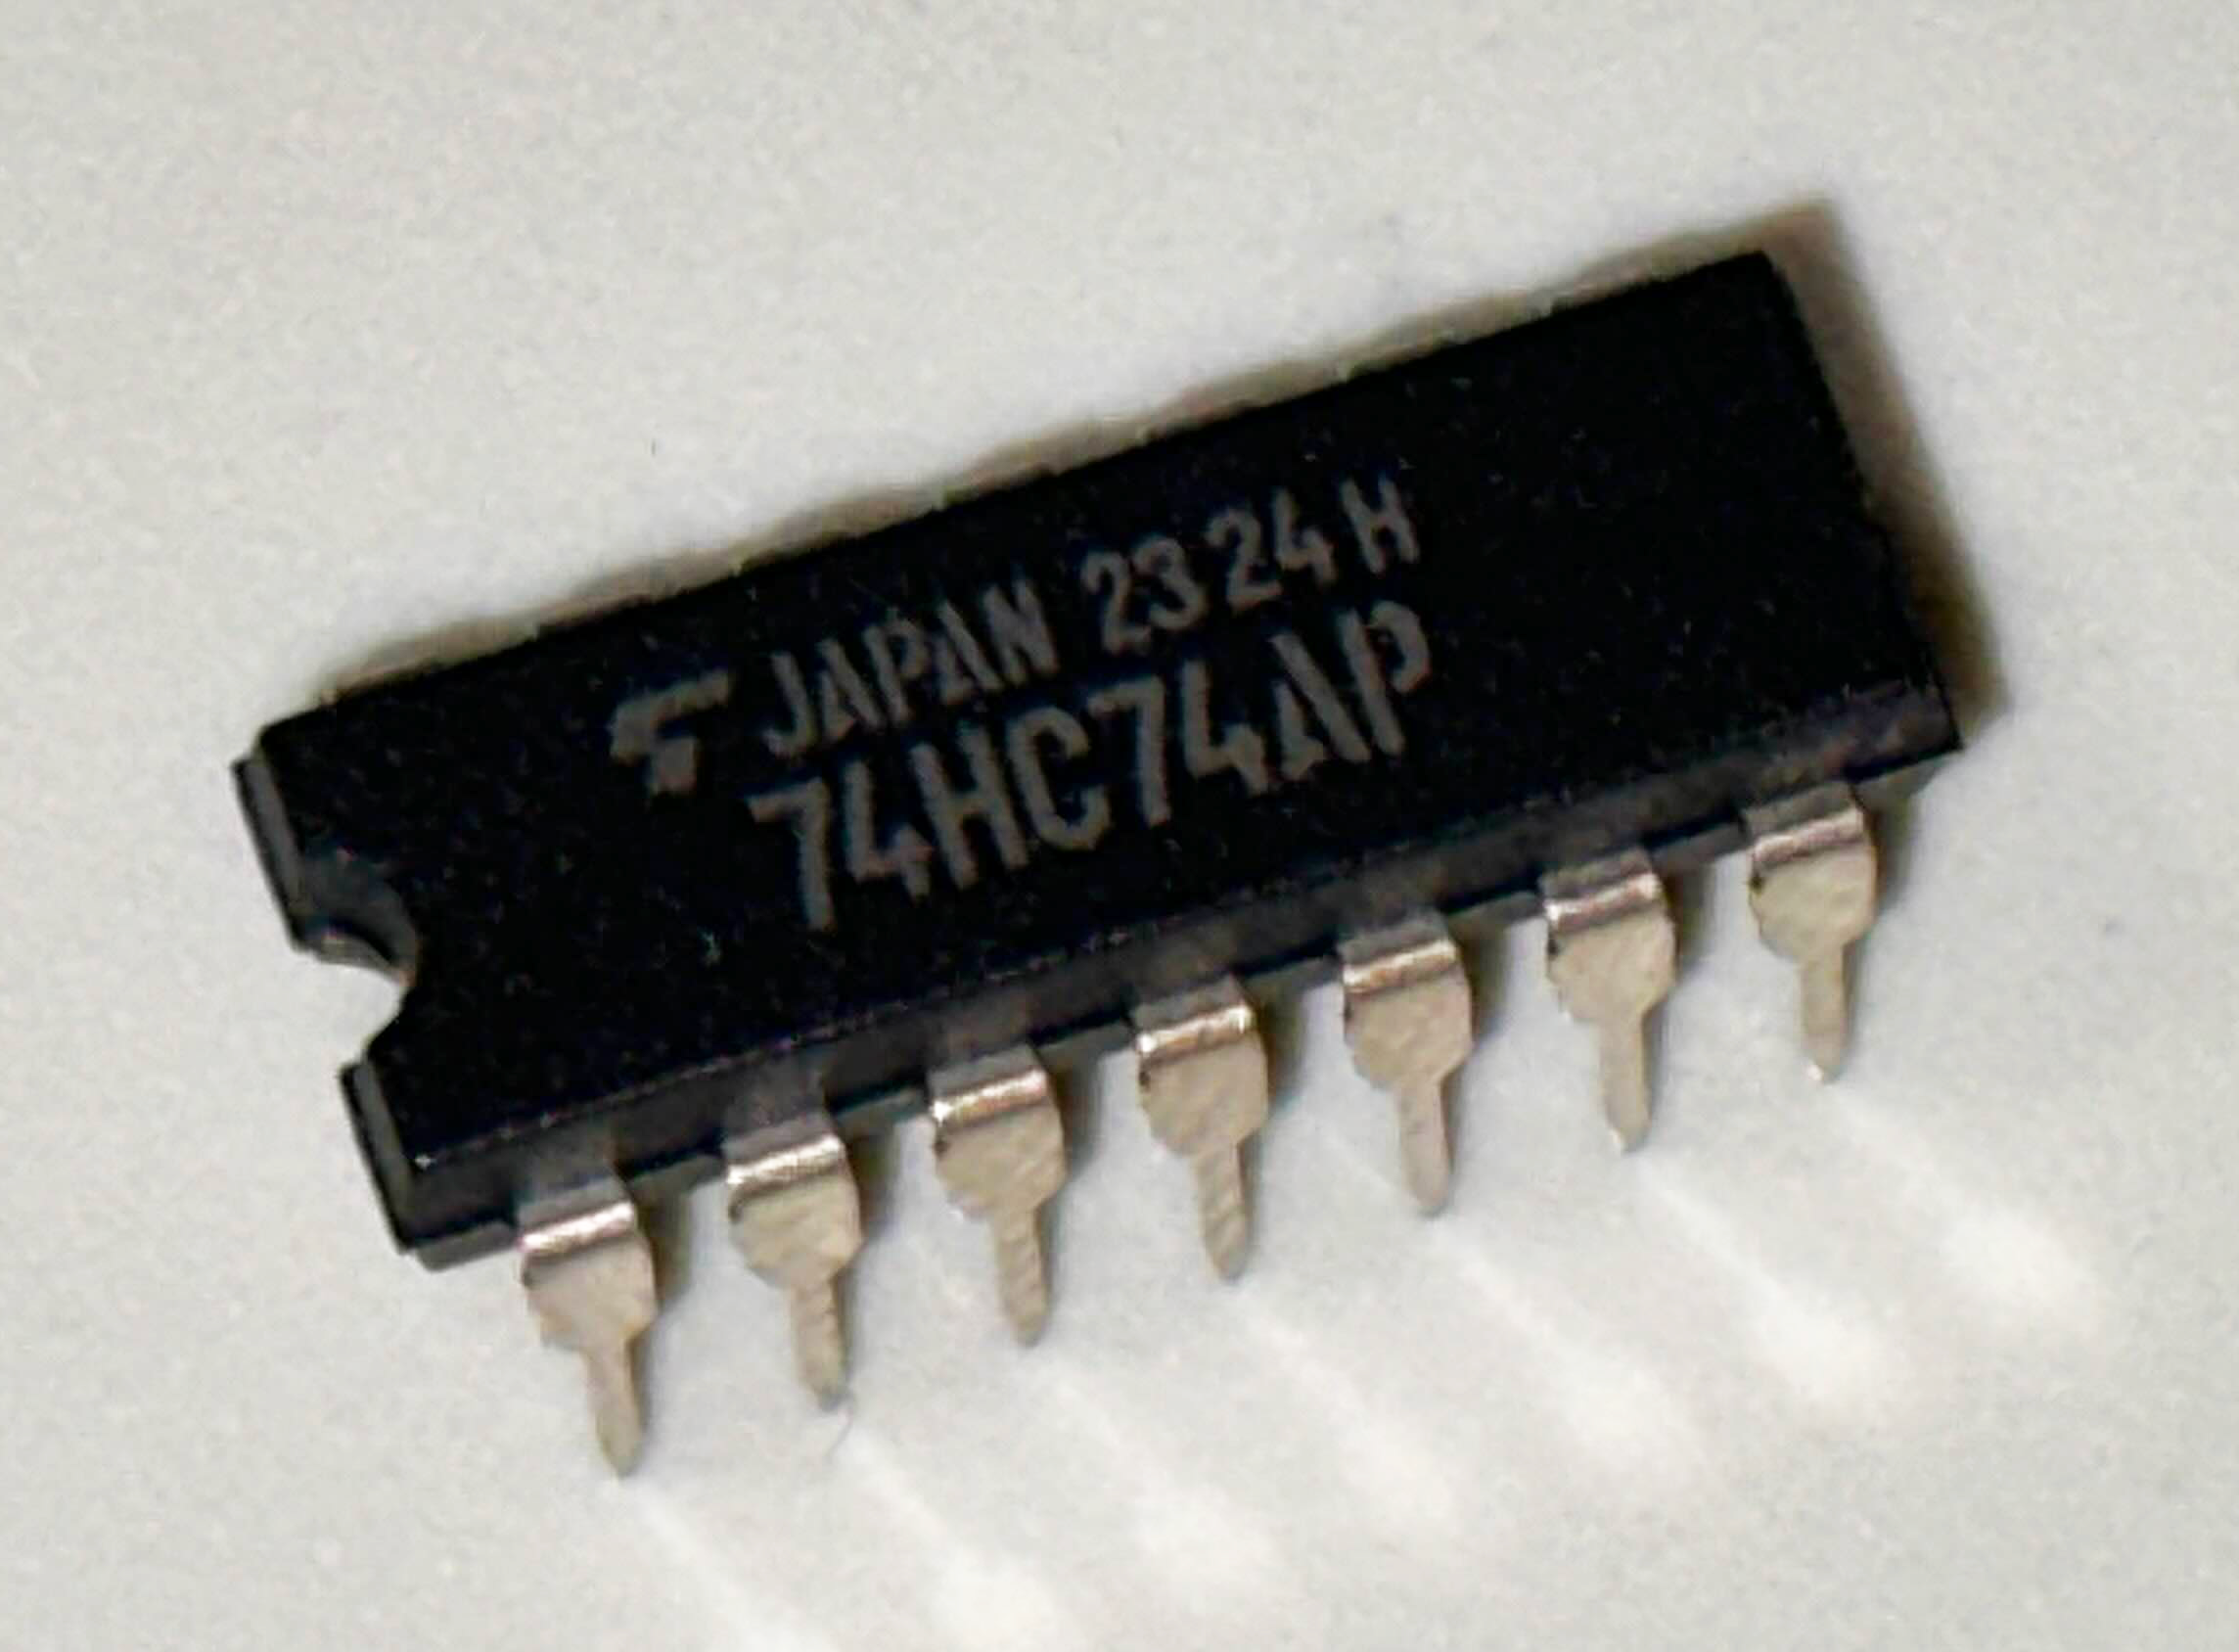
\includegraphics[keepaspectratio, width=\linewidth]{figure/ic.png}
        \caption{ICの外観}
        \label{fig:ic_overview}
    \end{minipage}
    \begin{minipage}[t]{0.45\linewidth}
        \centering
        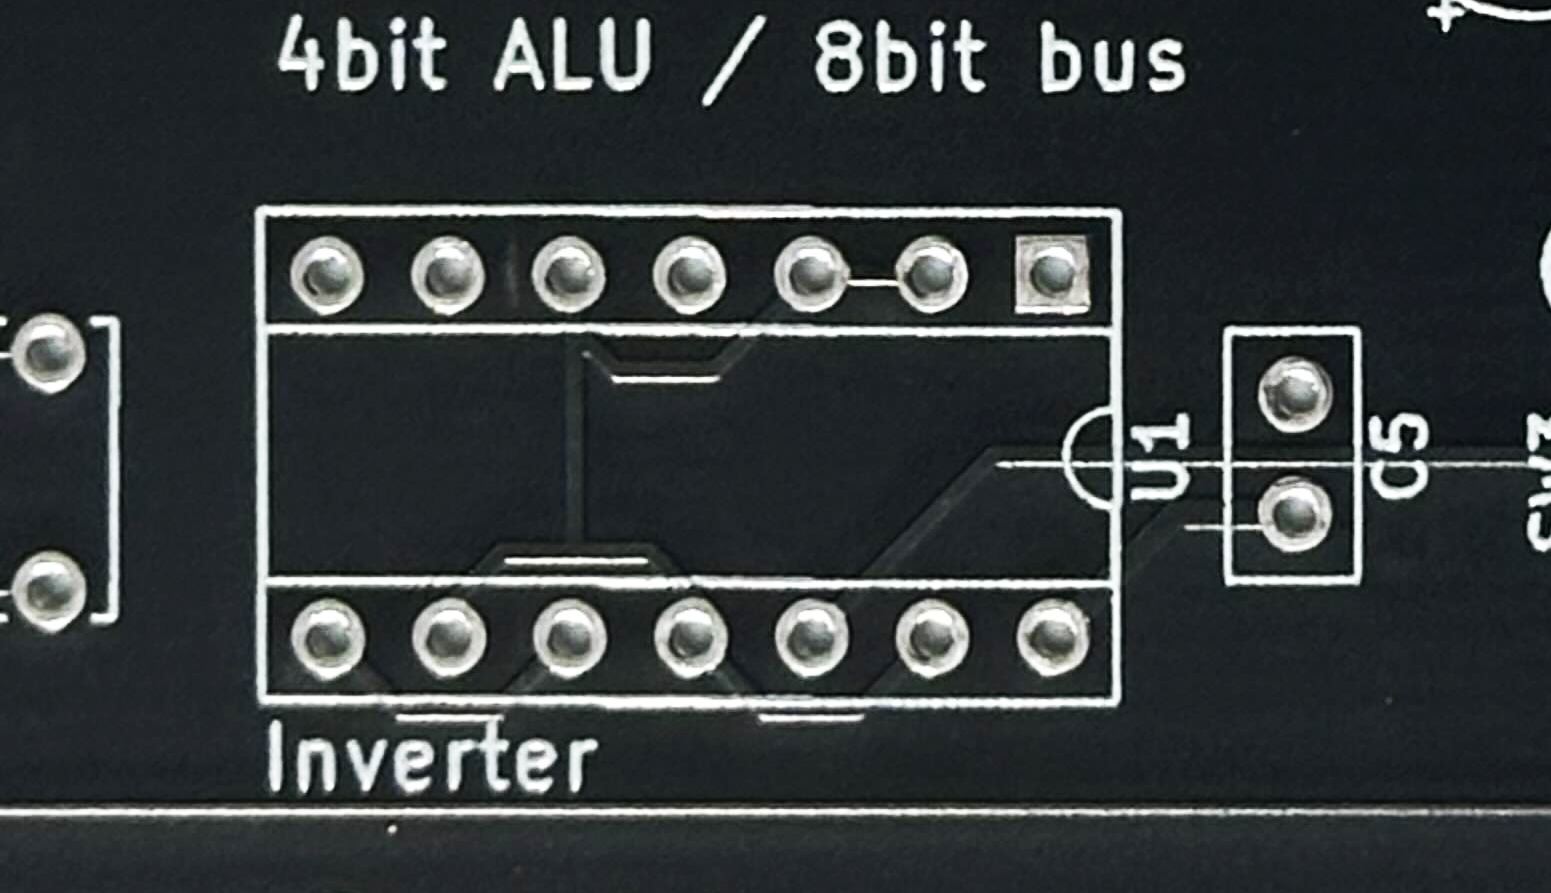
\includegraphics[keepaspectratio, width=\linewidth]{figure/ic_chip.png}
        \caption{基板上のICの印刷}
        \label{fig:ic_print}
    \end{minipage}
\end{figure}

\chapter{動作確認と使用}
はんだ付けが終わって完成してもTD4 CPUにはROMがないため、正しく動かない。そのためにまずはROMを用意する必要がある。

\section{ROM}
書籍ではROMは16個8PDIPスイッチを並べて製作していた。この方法はビジュアルとしては良いが結構部品代がかかるので断念した。
アドレスバスとデータバスを引き出しているので、ここに適当なROMを接続すれば良いが、筆者はArduinoでROMを作ることにした。

\begin{figure}[h]
    \centering
    \includegraphics[width=0.8\linewidth]{figure/td4_with_rom.png}
    \caption{Arduinoで作ったROMで動くTD4 CPU}
    \label{fig:td4withROM}
\end{figure}

\newpage

プログラムは以下の通り。

\lstinputlisting[language=c++]{td4_rom_arduino_new.ino}

Arduino UNO R4 WiFiで動作確認しているが、他でも動くと思う。あとはArduino側のD0-D7ピンをデータバスの0-7に、D8-D11をアドレスバスの0-3にそれぞれ接続し、+5VとVinを接続し、GND同士を接続してどちらかに電源を入れればプログラムが実行される。\par

\newpage

またPWRピンがあるがこれは入出力どちらでも使えるので、Arduino側から供給しても\footnote{Arduino側から供給する場合、電流制限に注意}、CPU側から供給しても良い。

\section{アセンブラー}
書籍ではアセンブル\footnote{人間に読みやすいように書かれたニーモニックを機械語に変換する処理}はハンドアセンブルのみが書かれていたが、めんどくさかったのでアセンブラーを作った。Linux上で動かすことを想定しているので、Windowsを使っている場合WSL上で行うことをお勧めする。

ビルドには\texttt{gcc, make, git, flex, bison}が必要なのでインストールする。Ubuntuを利用している場合は以下の通りになる。
\begin{lstlisting}
$ sudo apt update
$ sudo apt upgrade
$ sudo apt install gcc make git flex bison libbison-dev
\end{lstlisting}

ビルドは以下のコマンドで行う。
\begin{lstlisting}
$ cd ~
$ git clone https://github.com/nikachu2012/td4asm
$ cd td4asm
$ make all
\end{lstlisting}

test.asmというファイルををtd4asmと同じ場所に作り、中身を以下のようにする。
\begin{lstlisting}[caption=LEDちかちかさせるプログラム \texttt{test.asm}]
main: out 0b0011
      out 0b0110
      out 0b1100
      out 0b1000
      out 0b1000
      out 0b1100
      out 0b0110
      out 0b0011
      out 0b0001
      jmp main
\end{lstlisting}

以下のコマンドを実行するとtest.txtが作られる。
\begin{lstlisting}
$ ./td4asm -i test.asm -o test.txt -c
\end{lstlisting}

test.txtは以下のようになる。
\begin{lstlisting}
{0xb3, 0xb6, 0xbc, 0xb8, 0xb8, 0xbc, 0xb6, 0xb3, 0xb1, 0xf0, 0x00, 0x00, 0x00, 0x00, 0x00, 0x00}
\end{lstlisting}

このように、C言語の配列形式で機械語が出力される。

\chapter{最後に}

この本のPDFファイル、回路図などは以下のURLに用意した。

\centerline{\url{https://github.com/nikachu2012/td4cpu}}

また、すべての質問に答えられるかわからないが、このCPUの基板やアセンブラーについてわからない点などがあれば、奥付に記載のメールアドレスまで連絡していただければできるだけ質問に答える。

\vspace*{\fill}

\begin{tabular*}{\textwidth}{l}
    \noindent
    \textbf{\sffamily\Large 4bit CPU 製作基板\;説明書\normalsize}\vspace{3mm} \\
    \hline
    \begin{tabular}{@{}rrrl}
        2024年 & 11月 & 1日 & 初版第1刷発行\;\;(沼津高専\;第59回高専祭) \\
        % 2029年 & 1月 & 1日 & 初版第2刷発行\;\;(沼津高専\;第60回高専祭)
    \end{tabular} \\
    \\
    \begin{tabular}{@{}ll}
        \textbf{著者}  & \texttt{@nikachu2012} (荻野\;壮)                          \\
        \textbf{発行者} & \begin{tabular}{@{}l@{}}
                           \texttt{@nikachu2012} (荻野\;壮)  \\
                           \texttt{work@nikachu.net}
                       \end{tabular}               \\
        \textbf{発行所} & 沼津高専\;情報工学同好会(非公認)                          \\
        \textbf{印刷者} & 自分                                 \\
    \end{tabular} \\
    \hline
    Printed in Japan(多分)
\end{tabular*}


\end{document}
